\section{Methoden}

\subsection{Allgemeine Funktionsweise eines Spektrographen}
Mit Hilfe eines Spektrographen kann man Licht in seine Farben zerlegen. Dabei besteht ein Spektrograph im Wesentlichen aus folgenen Komponenten:

\begin{itemize}

\item Teleskop: Das Teleskop wird benötigt, um Licht zu sammeln und es zu fokussieren.

\item Spalt: Der Spalt schirmt unerwünschte Störquellen ab und sorgt dafür, dass am Dispersionselement ankommende Strahlung im besten Fall von einem Punkt ausgeht, da sich sonst die Auflösung verringert. Dabei kann die Spaltbreite allerdings nicht belibig klein gewählt  werden, da dadurch natürlich auch die Intensität des Lichts abnimmt. Deshalb muss hier ein Optimum gefunden werden.

\item Kollimator: Der Kollimator erzeugt aus dem einfallenden Licht paralleles Licht.

\item Dispersionselement: Das Dispersionselement ist der Hauptbestandteil des Spektrographen. Es trennt das Licht in Abhängigkeit von der Frequenz. Dabei kann es ein Prisma, oder auch ein Gitter sein. (Das Prisma trennt das Licht auf Grund der Frequenzabhängigkeit der Brechung, während die Trennung beim Gitter durch Interferenzeffekte hervorgerufen wird.)

\item Kamera-Objektiv: Das Kamera-Objektiv wird benötigt, um das durch das Dispersionselement erzeugte Spektrum auf den CCD-Detektor abbzubilden.

\item CCD-Detektor: Der CCD-Detektor digitalisiert schließlich das Bild des Spektrums.

\end{itemize}
Im Bamberger Spektrographen wird ein Blaze-Reflektionsgitter verwendet. (siehe Abb. \ref{fig:101} und \ref{fig:102} ) Dieses hat regelmäßig angeordnete geneigte Furchen und bietet so den Vorteil, dass das Intensitätsmaximum in Richtung des dispergierten Lichtes verschoben wird. Laut \cite{ronomischesPraktikum} ergibt sich aus der Bedingung für konstruktive Interferenz und dem Huygensschen Prinzip:

\begin{equation}
d \cdot ( \sin(\alpha) + \sin(\beta) ) = \Delta s \overset{!}{=} n \cdot \lambda
\label{form:Interferenz}
\end{equation}
Dabei sind $\alpha$, $\beta$ und d wie in den Abb. \ref{fig:101} und \ref{fig:102} zu erkennen. $\Delta s$ ist  die Wegdifferenz, n die Beugungsordnung und $\lambda$ die Wellenlänge des Lichts. Mit Hilfe dieser Formel kann man durch Messung von $\beta$ $\lambda$ bestimmen.

Um die Qualität  eines Spektrums zu beurteilen, wird das spektrale Auflösungsvermögen $R$ mittels der Wellenlänge $\lambda$ und der zugehörigen Unschärfe $\Delta \lambda$ folgendermaßen definiert:

\begin{equation}
R = \frac{\lambda}{\Delta \lambda}
\end{equation}

Die Unschärfe $\Delta \lambda$  wird  dabei durch zwei Prozesse erzeugt:

\begin{itemize}

\item Beim Beugen des Lichts am Gitter kommt es zum Verwaschen der Linien. Das Auflösungsvermögen des Gitters beträgt $ R_{Gitter} = n \cdot N $, wobei $ N $ die Anzahl der beleuchteten Spalten ist.

\item Die Breite des Spalts führt dazu, dass beliebig nahe Punkte im Spektrum nicht mehr getrennt werden können. 

\end{itemize}

\begin{figure}
		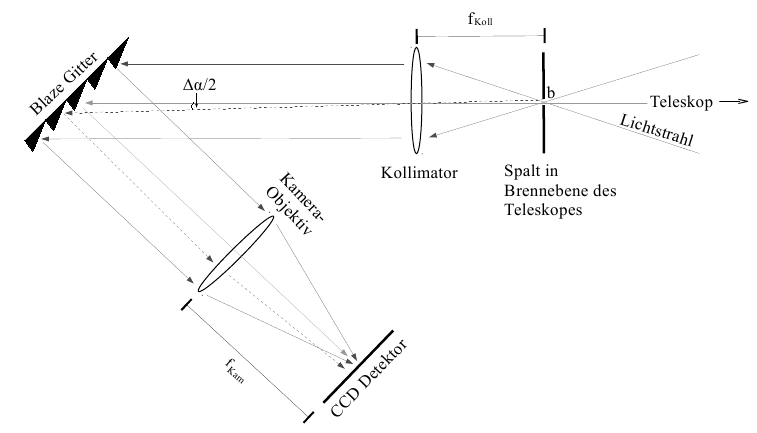
\includegraphics[width=.9\textwidth]{images/Abbildung101}
\caption{ Schematischer Aufbau eines Gitterspektrographen mit Blaze-Gitter }
\label{fig:101}
\end{figure}
\begin{figure}

        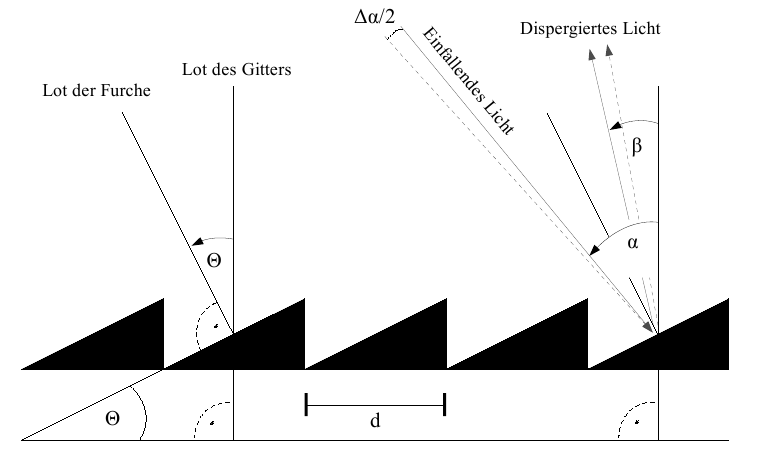
\includegraphics[width=.9\textwidth]{images/Abbildung102.png}
\caption{ Beispiel eines Blaze-Gitters und seiner charakteristischen Größen }
\label{fig:102}
\end{figure}
\begin{figure}

        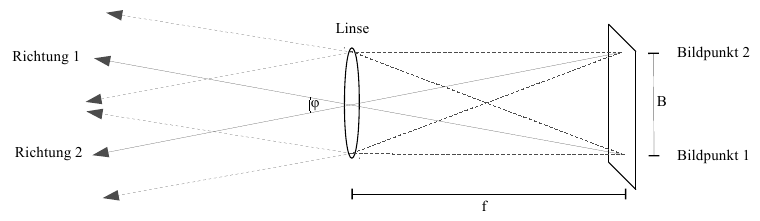
\includegraphics[width=.9\textwidth]{images/Abbildung103.png}
\caption{ Abbildungsmaßstab einer Linse }
\label{fig:103}
\end{figure}

\subsection{Die Rolle des Spalts}
Da der Spalt nicht unendlich schmal ist, trifft das Licht nicht perfekt parallel auf das Gitter. Deshalb variiert der Einfallswinkel $ \alpha $ um $ \Delta \alpha $, was letztendlich das Auflöungsvermögen verschlechtert.

\subsubsection{Wellenlängenunschärfe hervorgerufen durch endliche Spaltbreiten}
Für eine Linse (siehe Abb. \ref{fig:103}) gilt mit Hilfe der Kleinwinkelnäherung:

\begin{equation}
B = 2\cdot \sin{\frac{\phi}{2}} \cdot f = 2 \cdot \frac{\phi}{2} \cdot f = f \cdot \phi
\label{form:Kleinwinkel}
\end{equation}
Der vom Spalt \enquote{umspannte} Winkelbereich $\Delta \alpha $ beträgt nach \eqref{form:Kleinwinkel}:
\begin{equation}
\Delta \alpha = \frac{b}{f_{koll}}
\end{equation}
Leitet man \eqref{form:Interferenz} nach $ \alpha $ ab, erhält man:

\begin{equation}
\frac{d \lambda}{d \alpha} = \frac{d}{n} \cdot \cos{\alpha}
\end{equation}
Für hinreichend kleine $\alpha$ ergibt sich mit der Näherung $ \Delta \lambda = \frac{d\lambda}{d\alpha} \cdot \Delta \alpha $ :

\begin{equation}
\Delta \lambda = \frac{d}{n} \cdot \cos{\alpha} \cdot \frac{b}{f_{koll}}
\end{equation} 
Für das Auflösungsvermögen des Spalts ergibt sich mit $ R = \frac{\lambda}{\Delta \lambda} $ die Formel:

\begin{equation}
R_{Spalt} = \frac{n \cdot f_{Koll}}{d \cdot b \cdot \cos \alpha} \lambda
\end{equation}
Also ist die Auflösung auch durch den Spalt auf einen endlichen Wert begrenzt.

\subsubsection{Auflösung des Spektrographen}
Laut \cite{ronomischesPraktikum} ist die durch die Spaltbreite vorgegebene Auflöung typyscherweise wesentlich kleiner als die des Gitters. Deshalb kann in guter Näherung davon ausgegangen werden, dass für die Auflösung des gesamten Spektrographen gilt:

\begin{equation}
R = \frac{n \cdot f_{Koll}}{d \cdot b \cdot \cos \alpha} \lambda
\label{form:Auflösung}
\end{equation}
Um eine möglichst gute Auflösung zu erhalten, muss man also die Parameter aus \eqref{form:Auflösung} so wählen, dass $ R $ möglichst groß wird. Dies ist in der Praxis jedoch nur bedingt möglich. Die zwei einfachsten Maßnahmen, dies umzusetzen sind:

\begin{itemize}

\item Verkleinern der Spaltbreite $ b $

\item Beobachten in hohen Beugungsordnungen $ n $

\end{itemize}

\subsubsection{Optimierung der Auflösung des Spektrographen}
Beide oben genannten Maßnahmnen bringen auch Nachteile mit sich. So darf z.B. die Spaltbreite nicht zu klein gewählt werden, da Sterne die von der Erde aus beobachtet werden durch das Seeing eine nicht zu vernachlässigende Ausdehnung erhalten. Ein Stern beim durchschnittlichen Bamberger Seeing hat in der Fokalebene einen Durchmesser von $48.9 \mu \mathrm{m} $. Dieser Wert wäre also der kleinste mögliche Wert mit voller Lichteinstrahlung und somit der ideale Wert für die Blendenöffnung.

\subsection{Echelle-Spektrograph}
\subsubsection{Überlappung von Beugungsordnungen}
Verwendet man hohe Beugungsordnungen, überlappen sich diese meistens sehr stark. Im Folgenden soll als Beispiel berechnet werden, für welche Wellenlängen der Ordnungen $ n = $ 34, 46 und 58 Licht unter dem gleichen Ausfallswinkel  $ \beta $ gebeugt wird wie Licht der Wellenlänge $ \lambda_{33} = $ 6662.2686 $ \AA $ in der Ordnung $ n = $ 33. (Dabei sollen der Einfallswinkel $ \alpha $ und der Spaltabstand konstant gehalten werden.)\\

Da $\alpha$ und $d$ konstant gehalten werden und $\beta$ konstant sein soll, muss für das Licht verschiedener Wellenlängen $n_1 \cdot \lambda_1 = n_2 \cdot \lambda_2$ gelten. Somit folgt: 

\begin{equation}
\lambda_n = \frac{33}{n} \cdot \lambda_{33}.
\end{equation}
Dies ergibt für n = 34 $\lambda_{34} \approx 6466.3195 \AA$, für n = 46 $\lambda_{46} \approx 4779.4536 \AA$ und für n = 58 $\lambda_{56} = 3790.6011 \AA$.\\

Um diese Überlagerungen aufzuspalten, wird ein Echelle-Spektrograph verwendet.

\subsubsection{Funktionsweise eines Echelle-Spektrographen}

\begin{figure}
		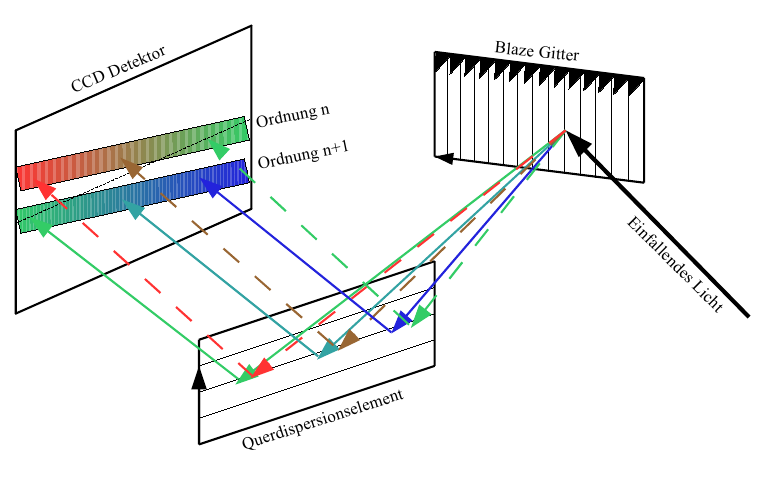
\includegraphics[width=.9\textwidth]{images/Abbildung104}
\caption{ Prinzip eines Echelle-Spektrographen }
\label{fig:104}
\end{figure}

fuck


\subsection{Vorübungen (Werden noch in andere Kapitel eingefügt! Hier nur Lager! Also bitte nicht ändern!!! :-) }

\subsubsection{Vorübung 4}
Es gilt:
\begin{equation}
R_{Spalt} = \frac{n\cdot f_{Koll}}{d\cdot b\cdot cos \alpha}\cdot \lambda
\end{equation}
Ersetze $\lambda$ durch $\lambda_n^0$:
\begin{equation}
R_{Echelle} = \frac{n\cdot f_{Koll}}{d\cdot b\cdot cos \alpha}\cdot \frac{d}{n}[sin \alpha + sin(2\Theta-\alpha)] = \frac{f_{Koll}}{b}\cdot [tan \alpha + \frac{sin(2\Theta-\alpha)}{cos \alpha}]
\label{blabla}
\end{equation}
Dieser Term enthält nur Variablen, die sich aus dem Versuchsaufbau als konstant ergeben. 
Setze Tabellenwerte ein:
\begin{equation}
R_{Echelle} = \frac{100 \cdot 10^{-3}m}{25 \cdot 10^{-6}m}\cdot [tan (73.2^{\circ}) + \frac{sin(53.8^{\circ})}{cos (73.2^{\circ})}] \approx 24416
\end{equation}

\subsubsection{Vorübung 5}
Ersetze Größen aus Gleichung (\ref{blabla}) durch die kameraseitigen Größen ($b \rightarrow 2b_{Pixel}$) aus dem Nyquist-Kriterium:
\begin{equation}
R_{CCD} = \frac{f_{Kamera}}{2b_{Pixel}}\cdot [tan \beta + \frac{sin(2\Theta-\beta)}{cos \beta}]
\end{equation}
Setze Tabellenwerte ein:
\begin{equation}
R_{CCD} = \frac{150\cdot10^{-3}m}{18\cdot10^{-6}m}\cdot [tan (53.8^{\circ}) + \frac{sin(73.2^{\circ})}{cos (53.8^{\circ})}] \approx 25000
\end{equation}
Die Auflösung der CCD-Kamera ist in der gleichen Größenordnung wie die des Spektrographen. 



\subsection{Durchführung der Messung}
Leon ist voll cool

\subsection{Datenreduktion}
Um die aufgenommenen Spektren am Computer untersuchen zu können, müssen sie zunächst kalibriert und reduziert werden. Dies wurde in diesem Versuch mit dem Programmpaket MIDAS (Munich Image Data Analysis System) durchgeführt. Zunächst wurden die Beugungsordnungen und deren Position auf dem CCD-Chip identifiziert. Dazu mussten mehrere Kalibrationen mit verschiedenen angegebenen Anzahlen von Beugungsordnungen durchgeführt werden, bis alle Beugungsordnungen korrekt identifiziert wurden. Der zweite Schritt bestand darin, den Pixeln auf dem CCD-Chip die entsprechenden Wellenlängen zuzuordnen. Dazu wurde das aufgenommene Spektrum der ThAr-Lampe mit einem Referenzspektrum verglichen, indem zwei im Referenzspektrum gegebene Linien und deren Beugungsordnungen in dem aufgenommenen Spektrum markiert wurden. Anhand dieser Daten konnte MIDAS dann die Wellenlängenkalibration durchführen.\
Die eigentliche Reduktion der Daten wurde danach vorgenommen. In der Reduktion werden CCD-Effekte (Dunkelstrom, überbelichtete Pixel aufgrund von hochenergetischer kosmischer Strahlung) und in dem optischen Aufbau entstehendes Streulicht von der Aufnahme entfernt. Weiterhin wird eine Wellenlängenkalibration anhand des ThAr-Vergleichsspektrums durchgeführt und die einzelnen Beugungsordnungen extrahiert und in eindimensionale Datenarrays umgewandelt ('rebinning'). Es ist außerdem notwendig, den Einfluss der Blaze-Funktion durch eine Flatfield-Korrektur zu entfernen, um ein lückenloses Spektrum zu erzeugen. Schließlich werden noch die einzelnen Beugungsordnungen zu einem einzelnen Spektrum zusammengefügt und das kontinuierliche Spektrum auf eins normiert. Die Normierung wurde für unsere Messung jedoch nicht durchgeführt.  

\section{Auswertung}
\subsection{Bestimmung der Auflösung}
Aus dem aufgenommenen Spektrum der ThAr-Lampe kann empirisch eine Auflösung bestimmt werden, indem für mehrere Linien der Quotient aus Wellenlänge und Halbwertsbreite bestimmt und gemittelt wird. Dies wurde in MIDAS durchgeführt, indem über die Peaks eine Gaußfunktion gefittet wurde. Die erhaltenen Daten sind in Tabelle \ref{tab:3a}, Seite  \pageref{tab:3a} enthalten. Der Wert wurde also über die Formel
\begin{equation}
R_{Emp} = \frac{\lambda}{b}
\end{equation}
bestimmt, wobei $\lambda$ die Wellenlänge und $b$ die Halbwertsbreite ist. Der aus diesen Werten bestimmte Mittelwert mit Standardabweichung ergibt sich zu:
\begin{equation}
R_{Emp} = 13663.3 \pm 2445.8
\end{equation}
Dieser Wert lässt sich auch von MIDAS direkt berechnen, wobei MIDAS das Ergebnis
\begin{equation}
R_{Emp} = 12547.7 \pm 3398.3
\end{equation}
ausgibt. Es ist anzunehmen, dass MIDAS eine weitaus größere Anzahl von Linien für die Berechnung des Werts verwendet, deswegen ist dieser Wert trotz der größeren Standardabweichung als genauer anzunehmen.
\\
Es wurden bereits aus theoretischen Überlegungen Auflösungen für das Spektrometer und die CCD-Kamera bestimmt:
\begin{equation}
R_{Echelle} = 24416
\end{equation}
\begin{equation}
R_{CCD} =  25000
\end{equation}
Man sieht, dass die empirisch bestimmte Auflösung zwar in der gleichen Größenordnung, aber um ca. einen Faktor 2 kleiner ist.

HIER ETWAS SCHLAUES DAZU SCHREIBEN WARUM DAS SO IST

\subsection{Auswertung der Spektren}
\subsubsection{Die Harvard-Klassifikation}
Sterne können anhand ihres Spektrums in verschiedene Typen eingeteilt werden. Diese Einteilung heißt Harvard-Klassifikation und ordnet Sterne in die Klassen O,B,A,F,G,K, oder M ein (fränkischer, geschlechtsneutraler Merkspruch: 'Ohne Bier ausm Fass gibts ka Maß'). Eine Einteilung der Sterne in diese Klassen ist anhand des Vorhandenseins bestimmter Absorptionslinien möglich. Der Unterschied zwischen Spektren von verschiedenen Sternen ist vor allem durch die Temperatur der Sterne bedingt. Die Linien werden durch Absorption von Photonen durch die Elektronen der Atome in der stellaren Atmosphäre erzeugt. So wird z.B. die Helium I - Linie durch Absorption von Photonen durch He-Atome im angeregten Zustand erzeugt. Um die He-Atome anzuregen, muss die Temperatur aber entsprechend hoch sein, sodass diese Linie in kalten Sternen nicht zu sehen ist. Bei höherer Temperatur sind auch mehr Atome im angeregten Zustand, womit mehr Photonen absorbiert werden und die Linie eine stärkere (bzw. niedrigere) Intensität erhält. Wenn die Temperatur weiter ansteigt, werden die He-Atome jedoch ionisiert und können daher keine Photonen mehr absorbieren, womit die Intensität der Linie wieder abnimmt (bzw. größer wird). Mit diesen Mechanismen lässt sich auch das Verhalten anderer Linien (Ca I, He II, Fe I) erklären. Eine graphische Übersicht ist in Abb. \ref{fig:Harvard} dargestellt.
\\
Anhand der Absorptionslinien im Spektrum kann man nun einige Kriterien zur Einteilung angeben:
\begin{itemize}
\item Wenn das Spektrum nur wenige, dafür sehr intensive Linien zeigt, ist der Stern heiß, also in den Klassen O, B oder A.
\item Wenn das Spektrum sehr viele Linien zeigt, ist der Stern kalt, also in den Klassen F, G, K oder M.
\end{itemize}

WARUM IST DAS SO NACHFRAGEN

\begin{table}
\centering
\begin{tabular}{c|c|c|c|c|c|c}

 & He II & He I & Fe II & Ca I & G-Band & TiO-Band \\ 
\hline 
O & • & • &  &  &  &  \\ 
\hline 
B &  & • &  &  &  &  \\ 
\hline 
A &  &  &  &  &  &  \\ 
\hline 
F &  &  & • &  &  & \\ 
\hline 
G &  &  &  & • & • &  \\ 
\hline 
K &  &  &  & • &  &  \\ 
\hline 
M &  &  &  & • &  & • \\ 
\end{tabular}
\caption{Existenz von Absorptionslinien nach Spektralklasse}
\label{tab:Spektral}
\end{table}

Mit diesen beiden Kriterien und den in Tabelle \ref{tab:Spektral} dargestellten Linien kann man Sterne sehr gut anhand ihres Spektrums in Spektraltypen einordnen. Da die Übergänge zwischen Spektraltypen teilweise fließend sind, ist die so gefundene Einordnung aber manchmal nicht eindeutig und es muss eine gründlichere Untersuchung durchgeführt werden, für die Zwecke des Praktikums ist dies aber ausreichend.